
%%% Local Variables:
%%% mode: latex
%%% End:

\def\dx{.5cm}
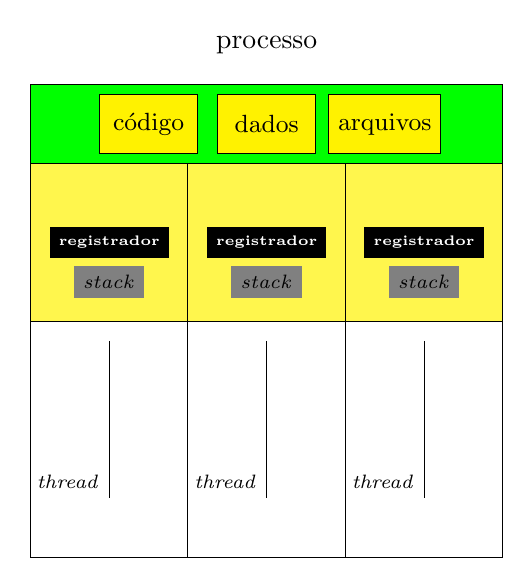
\begin{tikzpicture}
  \tikzset{resources/.style={minimum height=.75cm,minimum width=1.25cm,font=\small,fill=yellow,draw}}

  \node[fill=green,minimum width=6cm,minimum height=1cm,draw] at (0,0) (text) {};
  \node [above of=text] {processo};
  \node[resources] at (0,0) (data) {dados};
  \node[resources] (code) [left of=data,xshift=-\dx] {código};
  \node[resources] (files) [right of=data,xshift=\dx] {arquivos};

  \foreach \x in {-1,0,1} {
    \node[fill=yellow!70,minimum height=2cm,minimum width=2cm,draw] (dynamic\x) [below of=text,yshift=-.5cm,xshift=2*\x cm] {};
    \node[color=white,fill=black] (reg\x) at (dynamic\x)  {\bf\tiny registrador};
    \node[fill=gray] (stack\x) [below of=reg\x,yshift=.5cm] {\scriptsize\emph{stack}};
    \node[minimum height=3cm,minimum width=2cm,draw] (thread\x) [below of=stack\x,yshift=-1cm] {};
    \draw (2*\x cm,-5.5*\dx) -- +(0,-2cm) node[anchor=south east] {\scriptsize\emph{thread}};
  }
\end{tikzpicture}
